%%% LaTeX Template: Two column article
%%%
%%% Source: http://www.howtotex.com/
%%% Feel free to distribute this template, but please keep to referal to http://www.howtotex.com/ here.
%%% Date: February 2011

%%% Preamble
\documentclass[	DIV=calc,%
							paper=a4,%
							fontsize=11pt,%
							twocolumn]{scrartcl}	 					% KOMA-article class

\usepackage{lipsum}													% Package to create dummy text

\usepackage[english]{babel}										% English language/hyphenation
\usepackage[protrusion=true,expansion=true]{microtype}				% Better typography
\usepackage{amsmath,amsfonts,amsthm}					% Math packages
\usepackage[pdftex]{graphicx}									% Enable pdflatex
\usepackage[svgnames]{xcolor}									% Enabling colors by their 'svgnames'
\usepackage[hang, small,labelfont=bf,up,textfont=it,up]{caption}	% Custom captions under/above floats
\usepackage{epstopdf}												% Converts .eps to .pdf
\usepackage{subfig}													% Subfigures
\usepackage{booktabs}												% Nicer tables
\usepackage{fix-cm}													% Custom fontsizes
\usepackage[utf8]{inputenc}
\usepackage[rightcaption]{sidecap} 
\usepackage{graphicx} %package to manage images


%%% Custom sectioning (sectsty package)
\usepackage{sectsty}													% Custom sectioning (see below)
\allsectionsfont{%															% Change font of al section commands
	\usefont{OT1}{phv}{b}{n}%										% bch-b-n: CharterBT-Bold font
	}

\sectionfont{%																% Change font of \section command
	\usefont{OT1}{phv}{b}{n}%										% bch-b-n: CharterBT-Bold font
	}



%%% Headers and footers
\usepackage{fancyhdr}												% Needed to define custom headers/footers
	\pagestyle{fancy}														% Enabling the custom headers/footers
\usepackage{lastpage}	

% Header (empty)
\lhead{}
\chead{}
\rhead{}
% Footer (you may change this to your own needs)
\lfoot{\footnotesize \texttt{Thibaut EHLINGER} \textbullet ~Comparaison des algorithmes TCP}
\cfoot{}
\rfoot{\footnotesize page \thepage\ of \pageref{LastPage}}	% "Page 1 of 2"
\renewcommand{\headrulewidth}{0.0pt}
\renewcommand{\footrulewidth}{0.4pt}



%%% Creating an initial of the very first character of the content
\usepackage{lettrine}
\newcommand{\initial}[1]{%
     \lettrine[lines=3,lhang=0.3,nindent=0em]{
     				\color{DarkGoldenrod}
     				{\textsf{#1}}}{}}



%%% Title, author and date metadata
\usepackage{titling}															% For custom titles

\newcommand{\HorRule}{\color{DarkGoldenrod}%			% Creating a horizontal rule
									  	\rule{\linewidth}{1pt}%
										}
										
										\renewcommand\thesubsubsection{}

\pretitle{\vspace{-60pt} \begin{flushleft} \HorRule 
				\fontsize{15}{15} \usefont{OT1}{phv}{b}{n} \color{DarkRed} \selectfont 
				}
\title{Comparaison des principaux algorithmes TCP}					% Title of your article goes here
\posttitle{\par\end{flushleft}\vskip 0.1em}

\preauthor{\begin{flushleft}
					\large \lineskip 0.1em \usefont{OT1}{phv}{b}{sl} \color{DarkRed}}
\author{Thibaut Ehlinger, }											% Author name goes here
\postauthor{\footnotesize \usefont{OT1}{phv}{m}{sl} \color{Black} 
					Université de Strasbourg 								% Institution of author
					\par\end{flushleft}\HorRule}

\date{22 octobre 2015}																			



%%% Begin document
\begin{document}
\maketitle
\thispagestyle{fancy} 			% Enabling the custom headers/footers for the first page 
% The first character should be within \initial{}
\initial{T}\textbf{CP (\textit{Transmission Control Protocol})} est une implémentation de la couche transport du modèle OSI. TCP étant omniprésent dans les réseaux actuels, il a donc souvent été étudié et réimplémenté, parfois parce qu'une implémentation présentait des faiblesses qui lui étaient inhérentes, parfois parce qu'aucune implémentation ne répondait à une problématique bien précise du réseau. Dans ce texte, nous étudierons tout d'abord les différentes implémentations historiques de TCP. Celles ayant été utilisées un jour ou l'autre mais qui sont ajourd'hui obsolètes car peu efficaces. Puis nous étudierons certains des algorithmes utilisés aujourd'hui, dans le but de comprendre quels sont les critères déterminants lors du choix de l'algorithme utilisé.

\section*{Les premières implémentations de TCP}
De TCP Tahoe à TCP Westwood, en passant par TCP Reno, nous allons présenter une série d'algorithmes qui se sont globalement succédés, chacun étant dans la plupart des cas plus efficace que son prédecesseur.

\subsection*{Tahoe}
\subsubsection*{Slow start \& congestion avoidance}
Cette implémentation est citée pour la première fois en 1988 dans un article de Van Jacobson et Karels. C'est la plus simple et la moins efficace, tout types de problème confondus. Il implémente le \textbf{slow start}, la \textbf{congestion avoidance}, et le \textbf{fast retransmit}. 
Cela signifie qu'il double la taille de sa CWND à chaque RTT, jusqu'à atteindre le sstresh. A ce moment il passe en congestion avoidance, n'augmentant la taille de sa CWND que de 1 à chaque RTT. En cas de time out, ou d'ACK triplement dupliqué, $sstresh=\frac{CWND_{current}}{2}$, et on repasse en slow start.
\subsubsection*{Avantages et faiblesses}
Tahoe est déjà une réelle avancée, car il permet d'approximer très grossièrement la plus grosse taille de fenêtre d'émission possible, et il reste stable à moins qu'il n'y aie des congestions sur le réseau. Dans ce cas, Tahoe peut s'adapter au problème et diminuer la taille de sa fenêtre d'émission.

Néanmoins, la réinitialisation de la fenêtre d'émission à \textbf{1} à la moindre perte de paquet est une sous-estimation beaucoup trop importante. La taille moyenne de CWND est donc bien plus faible que ce qu'elle pourrait être optimalement.


\subsection*{Reno}
Reno résoud déjà grandement le problème de l'oscillation perpetuelle Slow Start/CA en ajoutant la notion de \textbf{Fast Recovery}.

\subsubsection*{Fast recovery}
Après un fast retransmit, au lieu de passer en Slow Start on applique :
$ sstresh=\frac{CWND}{2}, CWND=sstresh+3$. En fait on repasse directement en CA, tout en augmentant la taille de CWND de 3, en référence aux trois segments qui n'ont pas été reçus à cause des ACK dupliqués. En cas de time out néanmoins, on repasse en Slow Start. Cette stratégie permet en cas de perte de ne pas baisser drastiquement la taille de CWND, à moins d'un time out. Un time out est en fait plus grave qu'une simple perte de paquet. Il témoigne probablement d'une modification topologique du réseau ou bien d'une congestion importante, alors qu'une simple perte de paquet peut-être due à des évènements plus ponctuels, tels qu'un déséquencement ou une perte.

\subsubsection*{Faiblesses}
TCP Reno réagit bien au pertes de paquets quand elles se limitent à une par rafale. Quand par contre il y en a plusieurs par rafale, Reno est presque aussi inefficace que Tahoe, car il ne peut détecter qu'une seule perte de paquet à la fois.

De plus, il se peut qu'au sein d'une même rafale, l'émetteur aie le temps de passer en Fast Recovery, puis à nouveau en Congestion Avoidance, \textbf{deux fois}. Ce qui veut dire que si la fenêtre est trop grande et les pertes trop espacées au sein de cette fenêtre, la CWND peut-être divisée par 4.

\subsection*{New Reno}
New Reno peut détecter les pertes de paquets multiples et est, de fait, plus performant que Reno. En effet, New Reno garde une trace de tous les segments envoyés dans une rafale. Lorsqu'il détecte une perte, il \textbf{reste} en fast recovery tant que tous les segments de cette rafale n'ont pas été acquittés par le destinataire. New Reno est mieux que Reno en tout point.
\subsubsection*{Problèmes}
Puisque les pertes ne sont détectées que par les duplications d'acquittements, il faut tout de même attendre un timeout entier pour détecter toutes les pertes. 
\subsection*{SACK}
\subsubsection*{ACK sélectifs}
SACK permet de nommer les segments non-reçus, contrairement à Reno qui se contente de dupliquer les acquittement. Cela permet de récupérer plus vite les paquets perdus.
\subsubsection*{Variable \textit{pipe}}
En Fast Recovery, SACK initialise une variable \textit{pipe}. C'est une estimation du nombre de paquets qui sont encore dans le réseau. Si SACK reçoit une duplication d'ACK, il incrémente pipe. Il le décrémente pour toute nouvelle transmission ou nouvel ACK. Quand $ pipe < CWD$, il renvoie tous les segements qui n'ont pas été acquittés. Cela permet de renvoyer plusieurs segments perdus en moins d'un RTT.
\subsubsection*{Problèmes de SACK}
SACK est nettement plus efficace que New Reno, mais il présente un défaut majeur : il doit être implémenté par l'émetteur \textbf{et} le récepteur, sinon il ne marchera pas.
\subsection*{Vegas}
\subsubsection*{Mécanisme de retransmission}
D'après les travaux de Lawrence Brakmo et Larry L. Peterson, deux chercheurs de l'université d'Arizona et concepteurs de Vegas, Reno et New Reno sont très peu performants en ce qui concernt les \textbf{time out}. En effet, ils ont mesuré que pour un RTT moyen de 500ms, il fallait approximativement \textbf{1100ms} à New Reno pour détecter un time out.\footnote{\begin{quote}\textit{In Reno, round trip time (RTT) and variance estimates are computed using a coarse-grained timer (around 500 ms), [...] we found that for losses that resulted in a timeout—usually due to two or more dropped segments in a RTT , the exact figure depends on the number of segments in 4 transit—it took Reno an average of 1100ms.}\end{quote}} Ce qui correspond effectivement à plus de deux RTT. Vegas mesure le temps écoulé entre l'envoi d'un segment et la réception de son acquittement. Et mesure ainsi dynamiquement les RTT.
Cela permet non seulement d'estimer le time out plus précisément et de perdre moins de temps en cas de réinitialisation déclenchée par un time out, mais non seulement de détecter les pertes et les déséquencements préventivement :
\begin{description}
	\item[En cas d'ACK dupliqué]{, on compare le nouveau RTT avec le RTT mesuré précédemment. Si elle est supérieure à Time Out value, on renvoie directement le segment suivant, sans attendre trois acquittements dupliqués.}
	\item[Après un ACK dupliqué]{on fait de même. En effet, il est moins couteux de renvoyer un segment que de perdre beaucoup de temps pour découvrir qu'il a été perdu. }
\end{description}
De plus, Vegas ne diminue la taille de sa CWND que si le dernier ACK renvoyé a été renvoyé \textbf{après} le dernier changement de taille de fenêtre. En effet on peut supposer que deux pertes peuvent avoir été provoquées par la même congestion et qu'il ne sert à rien d'y réagir deux fois.
\subsubsection*{Congestion avoidance}
Pour l'évitement de congestions, Vegas fait une estimation du débit \textit{attendu} et le compare avec le débit \textit{estimé}. Ensuite on fixe des seuils $\alpha<\beta$. Si la différence des débits est inférieure à $\alpha$ alors on augmente CWND linéairement, si elle est supérieure à $ \beta $, on la diminue linéairement.
\subsubsection*{Congestion avoidance}
En Slow Start, Vegas n'augmente exponentiellement que tout les RTT, donc moins fréquemment que ses comparses. De plus, on fixe expérimentalement un seuil $\gamma$. Si la différence entre le RTT \textit{estimé} et le \textit{attendu} est inférieure à ce $\gamma$, on repasse en CA.
\subsubsection*{Aggressivité}
La courbe de Vegas est donc très ronde puisque l'algorithme tente d'anticiper les problèmes de congestion. Ces variations sont beaucoup plus lentes que Reno, par exemple. On dit que Vegas est \textbf{peu aggressif}. Contrairement à Reno ou à Tahoe, il ne tente pas de prendre le plus de bande passante que possible. Il en prend plus si il sent que le réseau lui permet. Si Reno intervient sur le même réseau que Vegas, alors les performances de Vegas vont diminuer considérablement, étant donné que Vegas diminuera de sa propre initiative son débit d'émission en amont de la congestion provoquée par Reno. Vegas cède en quelque sorte la priorité aux autres algorithmes cités précedemment.

\subsection*{Westwood}
Westwood a été conçu pour les réseaux connaissant un taux de perte de paquet important malgré une absence de congestion, tels que les réseaux sans fil. Comme ces pertes sont inhérentes au réseau, il ne sert à rien de compter directement les paquets perdus, car le même taux de paquet sera perdu quelque soit la taille de CWND. Du coup, Westwood fait une estimation du débit du réseau en divisant la taille d'un paquet envoyé par l'intervalle de temps entre les deux derniers acquittements. En cas de duplication d'ACK ou de time out, on se base sur cette estimation pour fixer sstresh : $sstresh=\frac{BWE \times RTT_{min}}{segsize} $. Westwood se base donc sur le débit moyen du réseau au lieu de compter les pertes.

\subsubsection*{Aggessivité}
Westwood est "amical" (\textit{friendly}). D'après les fondateurs de Westwood, lorsqu'il est en concurrence avec Reno, il partage la connexion très équitablement. De plus, TCP Westwood est considérablement plus performant que Reno lorsqu'il y a des pertes de 1\% dans le réseau, ce qui est un taux crédible dans des réseaux non-filaires.

\section*{Les implémentations modernes de TCP}
\subsection*{BIC (\textit{\textbf{B}inary \textbf{I}ncrease \textbf{C}ongestion Control}}
BIC est une implémentation TCP optimisée pour les \textit{Long fat network}, c'est à dire les réseaux à grande latence et à à grand débit, tels que les réseaux satellitaires. Dans ces réseaux, il faut trouver la CWND optimale en provoquant le moins de perte de paquet possible. Pour ce faire, BIC fait une recherche binaire, recherche réputée pour sa complexitée logarithmique.

\subsubsection*{Protocole}
Pour procéder à sa recherche binaire, BIC enregistre $W_{max}$, la taille maximum de CWND avant le dernire Fast Recovery, et $W_{min}$, la taille de la fenêtre juste \textbf{avant} le dernier fast recovery. La moyenne de $W_{max}$ et $W_{min}$, $W_{temp}$ est utilisée comme CWND. On augmente CWND linéairement jusqu'à $W_{max}$. S'il y a perte de paquet, $W_{temp}$ devient le dernier $W_{max}$, sinon il devient le dernier $W_{min}$. La taille de la fenêtre $\{W_{max}\;W_{min}\}$ est divisée par deux à chaque itération. Afin de ne pas imposer de changement de débit trop violent au réseau, on plafonne l'augmentation de la CWND arbitrairement avec un indice $S_{max}$.

Quand CWND dépasse $W_{max}$, il faut trouver une nouvelle taille de fenêtre maximale. On entre alors en "Max probing" : on augmente d'abord CWND linéairement, de $S_{max}$, en supposant qu'il n'est pas loin, puis au bout d'un certain temps, s'il n'y a pas de perte, on suppose que $W_{max}$ est très élevé. Dans ce cas on augmente CWND de $N \times S_{max}$. N étant le nombre d'itérations de la phase Incremental Addition du max probing.

\subsection*{CUBIC}
BIC est certes avantageux pour les \textit{LFN}, mais il est très aggressif, dans le sens ou il augmente très rapidement et très fortement sa CWND. C'est normal, c'est le but de BIC. Pour des réseaux à faible débit ou faible RTT, cela peut-être néanmoins très contraignant.
\subsubsection*{Protocole}
Cubic se veut lui aussi souple et stable, mais beaucoup moins aggressif. La taille de CWND est déterminée par une fonction cubique : 

$W_{CUBIC} = C(t-K)^3 - W_{max}$, avec \textit{C} déterminé empiriquement, \textit{t} le temps écoulé depuis depuis la dernière réduction de fenêtre, $W_{max}$ la taille de la fenêtre juste avant la dernière réduction de fenêtre et 

$K = \sqrt[3]{W_{max}\times\frac{\beta}{C}}$, $\beta$ étant le facteur de réduction de la CWND lors de la dernière réduction.
Derrière cette fonction complexe se cachent plusieurs fait :
\begin{description}
\item{La fonction est \textbf{cubique}, donc elle croît rapidement puis se stabilise autour de la $W_{max}$, pour recroître rapidement.}
\item{Elle dépend de l'intervalle de temps écoulé depuis la dernière réduction ce qui signifie que \textbf{tous} les processus Cubic TCP d'un même réseau croîtront à la même vitesse, garantissant l'équité de l'algorithme envers différents agents TCP.}
\item{Si le RTT est faible, la fonction croît lentement. Ce qui résoud le problème d'aggressivité posé posé par BIC, car CUBIC est "amical" envers toutes les implémentations de TCP.} 	
\end{description}

\begin{figure}[h]
    \centering
    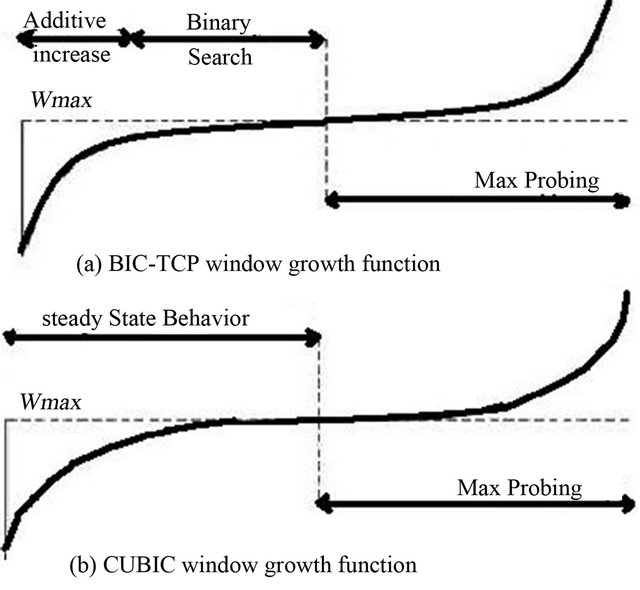
\includegraphics[width=0.5\textwidth]{Compound_vs_BIC}
    \caption{Sur ce schéma, on voit que CUBIC est plus rond que BIC autour de $W_{Max}$}
    \label{fig:mesh1}
\end{figure}

\subsection*{Compound}
Compound (qui signifie en anglais \textit{compsé}) tient son nom du fait qu'il est un hybride entre deux algorithmes TCP. L'idée derrière ce principe est que si le lien est sous-utilisé, alors il faut augmenter la taille de CWND le plus rapidement possible, mais que s'il est pleinement utilisé, alors il faut limiter l'aggressivité de l'algorithme, afin de garantir le \textit{TCP fairness}.
La CWND est la somme de deux fenêtre : une \textit{delay-window} et une \textit{AIMD-Window}. Bien que AIMD (\textit{additive-increase/multiplicative-decrease}) ne soit pas traité dans ce texte, on peut noter que cet algorithme augmente linéairement et est divisé par un facteur fixé arbitrairement en cas de congestion. En cas de perte de paquet, et qu'on entre en congestion avoidance, la \textit{delay-window} prend de plus en plus d'ampleur selon un algorithme très similaire à TCP Vegas, tandis que la \textit{AIMD-Window} a de moins en moins d'importance puisqu'elle augmente désormais très lentement.

\section*{Y a-t-il un meilleur TCP?}
\subsection*{Critères}
Il y a trois critères pour comparer l'efficacité des algorithmes :
\begin{description}
\item[Son \textbf{équité} :]{si plusieurs agents de cet algorithme tournent sur un même réseau, vont-ils se partager la bande passante équitablement?}
\item[Sa \textbf{compatibilité} :]{cet algorithme va-t-il être trop aggressif ou trop pacifique face à d'autres algorithmes TCP sur le réseau?}
\item[Son \textbf{efficacité} :]{cet algorithme monopolise-t-il en moyenne une proportion suffisante du lien?} 	
\end{description}
\subsection*{Bilan}
De nombreuses simulations ont montré que les premiers algorithmes de TCP sont désormais obsolètes. Vegas est incompatible avec Reno, Tahoe est trop oscillant, Reno/New Reno mettent trop de temps à détecter les pertes multiples, SACK est difficile à mettre en place et Westwood présente certains défauts qui ont été corrigés dans Westwood+.

Pour les implémentations modernes de TCP, le choix de l'algorithme dépend de la topologie du réseau. En effet, BIC est conçu pour les \textit{Long Fat Network}, tandis que CUBIC réagit mieux sur les réseaux à faible latence. Il est donc conseillé d'expérimenter différentes implémentations sur le réseau cible et de regarder laquelle est la plus efficace, en fonction du critère que l'on priorise. L'équité par exemple paraît très importante sur un réseau très peuplé, la compatibilité le paraît encore plus si l'on n'est pas maître des autres agents utilisant le réseau. Enfin si c'est un réseau peu peuplé, alors on peut se baser sur l'efficacité de l'algorithme lorsqu'on l-e sélectionne.
\begin{thebibliography}{9}

\tiny{\bibitem{Brakmo94}
	Lawrence S. Brakmo, Sean W. O’Malley, Larry L. Peterson,
	\emph{TCP Vegas : New Techniques for Congestion Detection and Avoidance},
	SIGCOMM Comput. Commun. Rev.,
	1994
\bibitem{Grieco95}
	Luigi A. Grieco, Saverio Mascolo ,
	\emph{Performance Evaluation and Comparison of Westwood+, New Reno, and Vegas TCP Congestion Control },
	SIGCOMM Comput. Commun. Rev.,
	2004
\bibitem{Casetti02}
	Claudio Casetti, Mario Gerla, Saverio Mascolo, M. Y. Sanadidi, Ren Wang
	\emph{TCP Westwood: End-to-End Congestion Control for Wired/Wireless Networks},
	Wirel. Netw.,
	2002
\bibitem{Casetti02}
	Lisong Xu, Khaled Harfoush, Injong Rhee
	\emph{ Binary Increase Congestion Control (BIC) for Fast Long-Distance Networks},
	INFOCOM 2004. Twenty-third AnnualJoint Conference of the IEEE Computer and Communications Societies,
	2004
\bibitem{Rhee05}
	Injong Rhee, Lisong Xu,
	\emph{CUBIC: A New TCP-Friendly High-Speed TCP Variant},
	SIGOPS Oper. Syst. Rev.,
	2008
\bibitem{compound1}
	Kun Tan, Jingmin Song, Qian Zhang, Murari Sridharan
	\emph{A Compound TCP Approach for High-speed and Long Distance Networks },
	INFOCOM 2006. 25th IEEE International Conference on Computer Communications. Proceedings		,
	2006
\bibitem{Site01}
	\emph{BIC and CUBIC}
	http://research.csc.ncsu.edu/netsrv/?q=content/bic-and-cubic}

\end{thebibliography}
\end{document}